\documentclass[]{beamer}
\usepackage[utf8]{inputenc}
\usepackage{hyperref}
\usepackage{listings}
\lstset{
    basicstyle=\fontsize{10}{12}\selectfont\ttfamily,
    keywordstyle=\color{blue},
    breaklines=true,
    showtabs=false,
    showstringspaces=false,
    numberstyle=\tiny\color{mygray}
}
% \usepackage[french]{babel}
% \uselanguage{French}
% \languagepath{French}
\usepackage{pslatex}        % for better PDF on screen
%\usepackage{textcomp}

% \usetheme{AnnArbor}
% \usetheme{Antibes}
% \usetheme{Berkeley}
%\usetheme{Berlin}
%\usetheme{Boadilla}
\usetheme{CambridgeUS}
% \usetheme{Copenhagen}
%\usetheme{Dresden}
%\usetheme{Frankfurt}
%\usetheme{Goettingen}
%\usetheme{Hannover}
%\usetheme{JuanLesPins}
%\usetheme{Marburg}
%\usetheme{Montpellier}
%\usetheme{PaloAlto}
%\usetheme{Pittsburgh}
%\usetheme{Rochester}
%\usetheme{Singapore}
%\usetheme{Szeged}
% \usetheme{Warsaw}



% Set Color ==============================
% Custom colors tested with CambridgeUS.
% If you want a nice looking presentation,
% simply comment this section.
% \usepackage{xcolor}

% http://www.computerhope.com/htmcolor.htm
% \definecolor{gold}{HTML}{FDD017}
% \definecolor{deep sky blue}{HTML}{3BB9FF}
% \definecolor{light sky blue}{HTML}{82CAFA}
% \definecolor{casesBlue}{HTML}{0072b8}
% 
% \makeatletter
% \definecolor{mybackground}{HTML}{82CAFA}
% \definecolor{myforeground}{HTML}{0000A0}
% 
% \setbeamercolor{normal text}{fg=black,bg=white}
% \setbeamercolor{alerted text}{fg=red}
% \setbeamercolor{example text}{fg=black}
% 
% \setbeamercolor{background canvas}{fg=myforeground, bg=white}
% \setbeamercolor{background}{fg=myforeground, bg=mybackground}

% \setbeamercolor{palette primary}{fg=black, bg=gold}
%       \setbeamercolor{palette secondary}{fg=black, bg=gray!20!white}
% \setbeamercolor{palette secondary}{fg=white, bg=casesBlue!80!gold}
% \setbeamercolor{palette tertiary}{fg=white, bg=casesBlue}
%       \makeatother

% Set Color ==============================




% Force full screen
% \hypersetup{pdfpagemode=FullScreen}

% Navigation menu
% disable options by commenting appropriate line
\setbeamertemplate{navigation symbols}{%
    \insertslidenavigationsymbol
    \insertframenavigationsymbol
    \insertsubsectionnavigationsymbol
    \insertsectionnavigationsymbol
    \insertdocnavigationsymbol
    \insertbackfindforwardnavigationsymbol
}


% contenu de la page de titre
\title[Introduction to MONARC]{Introduction to MONARC}
\subtitle{Optimised Risk Analysis Method}
\author[Team CASES]{Security Made In Lëtzebuerg / CASES}
\institute[]{\href{https://www.cases.lu}{Cyberworld Awareness and Security Enhancements Services}}
\date{February 12, 2020}
\logo{
\includegraphics[height=0.5cm]{../images/logo-cases.png}}
\newsavebox{\logoA}
\newsavebox{\logoB}
\savebox{\logoA}{
\includegraphics[width=3.0cm]{../images/logo-web-cases_lu.png}}
\savebox{\logoB}{
\includegraphics[width=3.0cm]{../images/logo-monarc-2.png}}
\titlegraphic{%
  \raisebox{.5\dimexpr\ht\logoB-\ht\logoA}{\usebox{\logoA}}% raise smaller logo into position
  \hspace*{5cm}%
  \usebox{\logoB}
}
% End of preamble




\begin{document}
\begin{frame}
    \titlepage
\end{frame}



% --------- Summary ---------
\setcounter{tocdepth}{1}
\begin{frame}
    \frametitle{Content at glance}
    \tableofcontents
\end{frame}
\setcounter{tocdepth}{4}
% ----------------------------



%
% SECTION: Security Made In Lëtzebuerg
%
\section{Who we are}
\begin{frame}
    \frametitle{Security Made In Lëtzebuerg (SMILE)}
    \begin{center}
        \begin{itemize}
            \item GIE - Groupement d’Intérêt Economique;
            \item 2003: Cyberworld Awareness and Security Enhancements Services (\textbf{CASES});
            \item 2007: Computer Incident Response Center Luxembourg (\textbf{CIRCL});
            \item 2010: SMILE (gie);
            \item 2017: Cybersecurity Competence Center (\textbf{C3}).
        \end{itemize}
    \end{center}
\end{frame}

\begin{frame}
    \frametitle{CASES}
    \framesubtitle{}
    \begin{block}{Mission}
        Promote information security by supporting Luxembourg administrations and SMEs.
    \end{block}
    Services:
    \begin{center}
        \begin{itemize}
            \item \textbf{awareness}, publications d'articles;
            \item \textbf{trainings}:
                introduction to cyber security for different professional audiences \footnote{\url{https://www.cases.lu/services/trainings.html}};
            \item \textbf{software}:
                MONARC, Diagnostic, Fit4Cybersecurity, MOSP, TACOS, etc.\footnote{\url{https://github.com/CASES-LU}}
        \end{itemize}
    \end{center}
\end{frame}




% 
% SECTION: What is MONARC?
%
\section{What is MONARC?}
\begin{frame}
    \frametitle{Summary}
    \begin{columns}[t]
        \begin{column}{5cm}
            \tableofcontents[sections={1-3}, currentsection, hideothersubsections]
        \end{column}
        \begin{column}{5cm}
            \tableofcontents[sections={4-5}, currentsection, hideothersubsections]
        \end{column}
    \end{columns}
\end{frame}
\subsection{An open source software}
\begin{frame}
\frametitle{An open source software}
\framesubtitle{}
    \begin{itemize}
        \item source code under \texttt{GNU Affero General Public License version 3} since 2017\footnote{\url{https://github.com/monarc-project}};
        \item application Web (SaaS, self-hosted, machine virtuelle);
        \item données sous licence \texttt{CC0 1.0 Universal (CC0 1.0) - Public Domain Dedication}\footnote{\url{https://creativecommons.org/publicdomain/zero/1.0}};
        \item données disponibles via une plateforme de partage\footnote{\url{https://objects.monarc.lu/organization/MONARC}}
    \end{itemize}
\end{frame}


\subsection{A method}
\begin{frame}
    \frametitle{Une méthode Structurée, Itérative et Qualitative}
    \framesubtitle{}
    \begin{columns}[t]
        \column{6.0cm}
        \begin{figure}
        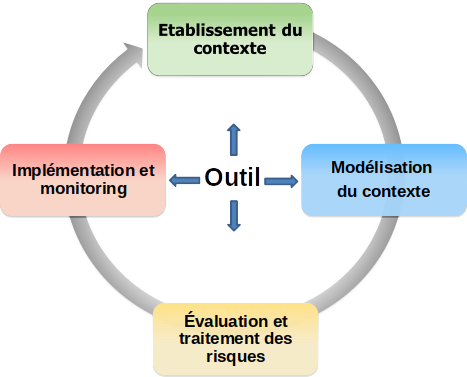
\includegraphics[width=6.0cm]{./images/MONARC-method-1.png}
        \end{figure}
        \column{6cm}
        \begin{itemize}
                \item Structurée: 1, 2, ..., n.
                \item Itérative: \textbf{Plan}, \textbf{Do}, \textbf{Check}, \textbf{Act}
                \item Qualitative: Impact/Conséquence, Menace, Vulnérabilité
        \end{itemize}
        \end{columns}
\end{frame}


\begin{frame}
    \frametitle{}
    \framesubtitle{Une gestion automatisée et simplifiée}
    \begin{center}
        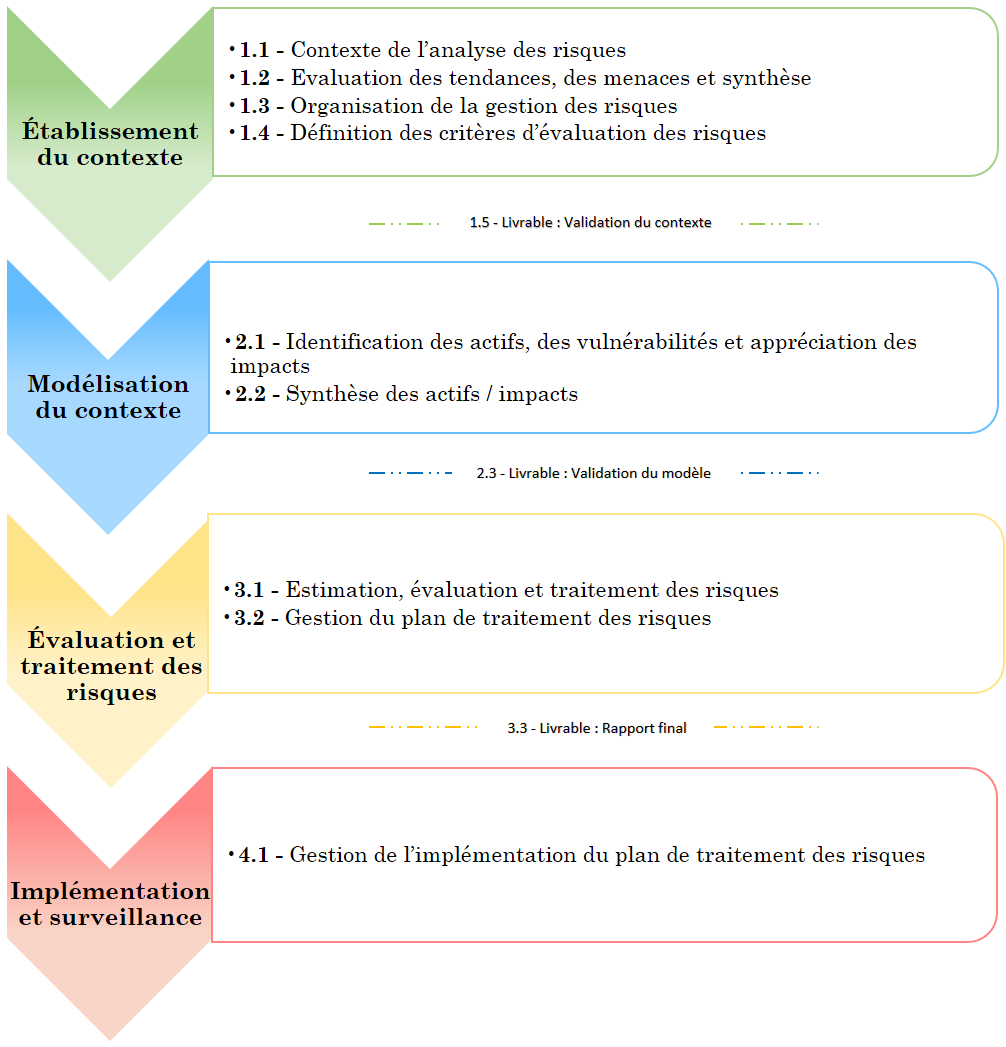
\includegraphics[scale=0.5]{./images/MONARC-method-2.png}
    \end{center}
\end{frame}


\begin{frame}
    \frametitle{Gestion de risques construite autour de la norme ISO/IEC 27005:2011}
    \framesubtitle{}
    \begin{block}{Risques de l’information}
        $$R = I \times M \times V$$
        \begin{itemize}
            \item Impact on CID;
            \item secondary assets.
        \end{itemize}
    \end{block}


    \begin{block}{Risques opérationnels}
        $$R = I \times P$$
        \begin{itemize}
            \item Impact on ROLFP. Brut/Net;
            \item primary assets
        \end{itemize}
    \end{block}
\end{frame}


\begin{frame}
    \frametitle{Optimisations}
    \framesubtitle{}
    \begin{block}{Une méthode optimisée}
    Héritage, portée des objets, modèles, livrables.
    \end{block}
\end{frame}




%
% SECTION: Run-through of the method
%
\section{Run-through of the method}
\begin{frame}
    \frametitle{Summary}
    \begin{columns}[t]
        \begin{column}{5cm}
            \tableofcontents[sections={1-3}, currentsection, hideothersubsections]
        \end{column}
        \begin{column}{5cm}
            \tableofcontents[sections={4-5}, currentsection, hideothersubsections]
        \end{column}
    \end{columns}
\end{frame}
\subsection{Method...}
\begin{frame}
    \frametitle{Title...}
    \framesubtitle{}
\end{frame}




%
% SECTION: Discovery and usage of the tool 
%
\section{Discovery and usage}
\begin{frame}
    \frametitle{Summary}
    \begin{columns}[t]
        \begin{column}{5cm}
            \tableofcontents[sections={1-3}, currentsection, hideothersubsections]
        \end{column}
        \begin{column}{5cm}
            \tableofcontents[sections={4-5}, currentsection, hideothersubsections]
        \end{column}
    \end{columns}
\end{frame}
\subsection{A Web application}
\begin{frame}
    \frametitle{Une application Web}
    \framesubtitle{}
\end{frame}




%
% SECTION: New functionalities
%
\section{New functionalities}
\begin{frame}
    \frametitle{Summary}
    \begin{columns}[t]
        \begin{column}{5cm}
            \tableofcontents[sections={1-3}, currentsection, hideothersubsections]
        \end{column}
        \begin{column}{5cm}
            \tableofcontents[sections={4-5}, currentsection, hideothersubsections]
        \end{column}
    \end{columns}
\end{frame}

\begin{frame}
    \frametitle{Developments}
    \framesubtitle{New developments}
    \begin{itemize}
        \item registre GDPR (MONARC 2.9.0);
        \item gestion d'ensemble de recommendations (MONARC 2.9.0)
        \item Statement of Applicability;
        \item connexion avec MOSP.
    \end{itemize}
\end{frame}

\begin{frame}
    \frametitle{Developments}
    \framesubtitle{Futurs developments}
    \begin{itemize}
        \item LDAP;
        
    \end{itemize}
\end{frame}




%
% SECTION: Services
%
\section*{Services}
\begin{frame}
    \frametitle{Services related to MONARC}
    \begin{center}
        \begin{itemize}
            \item help at deploying;
            \item help at using;
            \item trainings;
            \item developments, feature requests.
        \end{itemize}
    \end{center}
\end{frame}




%
% SECTION: End of the presentation
%
\section*{End of the presentation}
\begin{frame}
    \frametitle{Fin de la présentation}
    \framesubtitle{}
    \begin{center}
        \begin{itemize}
            \item Thank you for listening.
            \item Contact: info@cases.lu
            \item \url{https://www.monarc.lu}
        \end{itemize}
    \end{center}
\end{frame}
\end{document}
